\documentclass[12pt,letterpaper]{article}

\usepackage{pslatex}
\usepackage{apacite}
\usepackage{url}
\usepackage{graphicx}
\usepackage{todonotes}
\usepackage{comment}

\usepackage{lineno}
\linenumbers

\usepackage[margin=1in]{geometry}


\usepackage[T1]{fontenc}
\usepackage[utf8]{inputenc}
%\usepackage{tgbonum}
%\usepackage{lmodern}
\usepackage{palatino}

\renewcommand\bibliographytypesize{\small}

\newcommand{\andrew}[1]{\textcolor{magenta}{\bf [Andrew: #1]}}
\newcommand{\rdh}[1]{\textcolor{red}{\bf [Robert: #1]}}


\title{Emergent Collective Sensing\\ in Human Groups}

\author{
Robert Hawkins (rdhawkins@princeton.edu)\thanks{Department of Psychology, Princeton University}\\
Andrew M. Berdahl (berdahl@uw.edu)\thanks{School of Aquatic and Fishery Sciences, University of Washington}\\
Alex ``Sandy'' Pentland (pentland@mit.edu)\thanks{MIT Media Lab}\\
Noah D. Goodman (ngoodman@stanford.edu)\thanks{Department of Psychology, Stanford University}\\
Joshua B. Tenenbaum (jbt@mit.edu)\thanks{Department of Brain and Cognitive Sciences, Massachusetts Institute of Technology}\\
P. M. Krafft (p.krafft@oii.ox.ac.uk)\thanks{Oxford Internet Institute, University of Oxford}
}

\date{}
\begin{document}


\maketitle
\vspace{-2em}

\begin{abstract}

%Copying successful individuals can be a highly effective way to improve your lot when you're lost in the weeds.


%People are able to copy successful individuals even when success is not readily observable. 

%At the same time, success is not always readily observable.

%While this strategy would seem to be rendered difficult when success is not readily observable, .

%What cognitive abilities enable people to succeed at identifying successful individuals to copy even in such cases when success is obscured or ambiguous.

%Here we argue that flexible agent-reasoning abilities underlie participants' abilities to selectively copy successful individuals in an environment where success can only be inferred from behavior.




%The study of behavioral mechanisms of collective intelligence general regards either rules of thumb or more sophisticated inferential mechanisms that enable 

%Many studies of collective intelligence have documented mechanisms 
%Some have   

%Collective intelligence is the study of 
% \todo[inline]{pk: we are confounding literature on small/large populations, as well as literature on collective intelligence versus cultural evolution}
% Groups of agents are capable of solving problems that no individual can solve alone. \andrew{Yes, but grouping can also enhance abilities that they already have on their own.  Not sure which is going on here...} 
A variety of simple strategies have been proposed to explain collective intelligence in both humans and non-human animals, such as copying successful individuals or copying when uncertain. 
Yet the cognitive abilities supporting these strategies in collectives remain poorly understood.
Here, we propose that social reasoning plays an important role, allowing latent properties like ``success'' to be flexibly inferred from outward behavior when there is no direct access to others' payoffs.
Such inferences allow social learning to be balanced with exploration. 
%While intelligent behavior emerges only at large group sizes for many nonhuman species (e.g. fish or insects), humans rapidly benefit from social interaction even in small teams. 
%In this paper, we take a comparative approach to identify candidate  mechanisms of social cognition that may account for distinctively human forms of collective intelligence. 
%While a variety of simple mechanisms have been proposed to account for 
%Despite its importance, human collective intelligence remains enigmatic.  
%We know what features are predictive of collective intelligence in human groups, but we do not understand the specific mechanisms that lead to the emergence of this distributed information processing ability. 
%In contrast, there is a well-developed literature of experiments that have exposed the mechanisms of collective intelligence in nonhuman animal species.
In Experiment 1, we designed a collective search paradigm for human participants, inspired by the nonhuman animal literature, and found that performance quickly improves as a function of group size. 
%for groups of up to six human participants.
In Experiment 2, we placed human participants in scenarios with artificial agents that were explicitly constructed to evaluate the role of two mechanisms: independent exploration and targeted copying based on social inferences about who is currently successful. 
%We further validated our experimental results by implementing these mechanisms in a computational model: a simulated agent equipped with these mechanisms explained human performance better than models relying on other simple heuristics that have been proposed for nonhuman animals.
Finally, in Experiment 3, we generalize these results to groups in a more complex and noisy environment.
Taken together, we find that even the most rudimentary human social cognition abilities afford robust and flexible use of social learning strategies.

\textbf{Keywords:}
  collective intelligence; distributed cognition;
  social cognition; social computation; online experiments
\end{abstract}

\section{Introduction}

%Social learning enable culture. allows things to be cumulative. it's important!

%Learn to preferentially copy successful individuals even when success must be inferred.

%in the animal literature, socila learning mechanisms have mostly bee studied as these strategies

%here are vatrious mechanisms tha thave been proposed
%these mechanismstic account have succesfully provided finew-groaunded analysical, explained collecitv ebavhior in a lot of caase. these stratgeies also cna mostly be explained by through behavioral associative learning (andrew social foraging ref)

%in parallel to all this, there has been a bunch of social cognition work about the way people make inference. there has bene a lot of work in social learning in cogsci, but mostly isn;t used ot explain big emergenyt things. mostly local


%tehre has been stuff about cognitive abilities predicting ermgey things, but this is generally about measuring things about individual that you can predict things tfrom rather than interactive mechanisms.


%in the present work, we aim ot ground the emergeny thing in the more immedaiate, cognitively orienteg mechanisms.

%in the cases where models are used in human collective intelligence, the models tend to be the same as animal behavior litearutre, in that reward is modeled as visible. not so much social inferece mechanisms. 


%meanwhile the cognitve sciene litatrure,a whic has also been interested in social learnk ,has tended ot think of things less as sttrategyie sand more as cognitive abilitesy---inferences that agents can make, theory of mind 

%gap: what if the actual reward is hidden. then what?

%all this social inference stuff is about latent properties of 

%infering prferences, goal, beliefs and desires. things you can't just read off someone's face

%look at a social foraging like task

%but without being able to actually observe what the rewards are there

%copy the successful. it's just so obvious! what if you don't know who is successful

%we know copy successful, but what happens when you don't have direct access to success. 

%its unknow how distirbuted searhc might work in humans where there is potential for more soiphisticated individual mechanisms. 

%what are the two or three main reuslts?

%people can do collective searhc, increas in gropu size

%use agent reasoning

%uniquely suited to this 

%associatve 


%\begin{quote}``A boat; hey, I've seen a boat! It passed by now two moments ago. It went...uh, this way; it went this way! Follow me!''\\
%-Dory in \textit{Finding Nemo}
%\end{quote}

Relying on others can be as risky as it is rewarding. 
Advice seekers must disentangle good advice from bad, and balance the potential benefits of shared wisdom against the cost of being pulled in different directions. 
A group where everyone is sensitive to ``who knows what'' can be quite effective at sharing information and solving problems together, but getting that meta-knowledge is not trivial. 
What cognitive abilities enable such achievements of collective intelligence?
%Yet discovering this information without explicit instructions requires making inferences from . 

 

%While much work from evolutionary biologists has focused on heuristic descriptions of behavioral rules used in social learning, recent work by cognitive scientists has turned towards understanding the meta-cognitive reasoning and cognitive abilities at play in human social learning. Rather than just studying where, when, and how social observation is employed in decision-making, these cognitive scientists have been interested in understanding the underlying domain-general mental representations people have at their disposal that enable these kinds of social learning in the first place. 

% Paragraph 1 topic sentence: collective intelligence is important and depends on 'social learning'
%From ant colonies to basketball teams, groups of agents are able to accomplish feats of intelligence beyond the reach of any individual.
%Groups are not only able to distribute complex computations across agents more effectively \cite{hutchins_cognition_1995} --- new emergent processes arise from interactions between agents. 
%When agents can observe and learn from one another, they no longer need to independently obtain all of their information from direct experience with the world. 
%Social learning thus allows the group as a whole to cumulatively build on individual successes, and is considered to be a key process driving collective intelligence \cite{boyd2011cultural,tomasello_natural_2014, laland2017darwin}. 

% Paragraph 2 topic sentence: social learning needs to be *selective* to be effective, and when/who heuristics are one way of achieving selectivity.
The study of social learning examines how people and other animals make use of information from others around them.
A large body of work in human and non-human animals has focused on what strategies, or heuristics, allow social learning to be effective \cite{laland_social_2004,hoppitt2013social,RendellFogarty___Laland11_CognitiveCulture,laland2017darwin}. 
Indiscriminate copying, for example, is not an effective strategy. 
As more individuals rely on imitation, rather than independent asocial learning, it becomes increasingly likely that a random target of copying is using outdated or inaccurate information, decreasing the mean performance of the group \cite{rogers_does_1988}.
For the group to benefit from social learning, imitation must be deployed selectively \cite{kameda2003does,boyd1995does,kendal2005trade}, both in choosing the appropriate time to learn from others (\emph{when} strategies) and choosing the appropriate individuals to learn from (\emph{who} strategies). 
For example, a ``copy-when-uncertain'' heuristic allows an agent to deploy social learning only when independent exploration becomes challenging, or a ``copy-successful-individuals'' heuristic allows an agent to filter out low-quality social information and target other agents most likely to increase their own fitness.

% Paragraph 3 topic sentence: to explain flexibility of human groups, however, we need to go deeper than bundles of heuristics to understand the underlying cognitive mechanisms (e.g. social inference)
Attention has increasingly turned from documenting evidence for individual heuristics to investigating the abilities underlying the flexible use of different strategies \cite{heyes2016blackboxing,kendal2018social}. 
Agents often use hybrid strategies, combining multiple sources of \emph{who} or \emph{when} information, or deploy different strategies in different contexts \cite{mcelreath_beyond_2008}.
Thus, it may be useful to view social learning behavior not as the application of an inventory of simple copying rules, but as arising from deeper cognitive abilities.
Especially in the case of humans, and some non-human primates, there has been substantial interest in the extent to which social learning relies on abilities like meta-cognition \cite{heyes2016knows} or theory of mind \cite{shafto2012learning} that go beyond pure associative learning \cite{behrens2008associative,heyes_whats_2012,heyes2012simple}.
These proposed abilities allow agents to maintain explicit representations of ``who knows'' and thus concentrate social learning on particularly knowledgeable individuals.
Similar cognitive abilities have been implicated in organization science as predictors of collective intelligence in small groups \cite{woolley2010evidence,engel2014reading}.

% Paragraph 4 topic sentence: these social inference mechanisms may be particularly important for understanding how we flexibly decide who to learn from in environments where we can't directly access others' rewards (i.e. pointing out unrealistic assumption of a lot of previous work in groups, where it's no wonder they were able to get away with simpler heuristics; copying the most successful is easy if there's a button you can press saying exactly how successful everyone is!)
We suggest that these social inference abilities may also help shed light on a puzzle raised by \emph{who} heuristics like ``copy-successful-individuals.''
Computational simulations \cite{schlag1998imitate,lazer2007network,rendell_why_2010} and human experiments \cite{mason2008propagation,mesoudi2008experimental,mason2012collaborative} typically provide agents the ability to directly observe the underlying payoffs of different agents (sometimes at a cost).
However, many real-world environments do not provide such direct access. 
Indeed, hiding payoffs can reverse the benefits of selective copying because the solutions of different agents cannot be compared \cite{wisdom_social_2013}.
Accounts of selective copying that rely on information about who is successful or knowledgeable must also provide an account of how agents \emph{come to know} this information.
While it is possible that associative learning allows agents to adopt particular external cues as proxies (e.g. visible health or wealth), social inference abilities may provide a more flexible alternative. 
Humans continually move between different contexts where success manifests in different observable behaviors: a reliable cue of success in one environment may not be reliable in another.
By inverting a generative model of behavior \cite<e.g.>{jara2016naive,baker2017rational}, agents can make context-sensitive predictions and flexibly infer the hidden success or knowledge of others.

% Paragraph 5 topic sentence: in fact, recent cognitive science has extensively worked out how these mechanisms work in *individual* social learning experiments, but implications for groups & collective intelligence remain unclear
This ability has been extensively studied in cognitive science.
Even young children are able to rapidly infer which partners are more trustworthy and knowledgeable than others, and prefer to learn from them \cite{wood2013whom,sobel2013knowledge,poulin2016developmental,mills2016learning}, % gweon2014sins, harris2018cognitive
 and adults can appropriately discount unreliable social information in their decision-making \cite{hawthorne2019reasoning,velez2019integrating,WhalenEtAl18_SensitivityToSharedInfo}.
However, this cognitive science literature has largely developed independently from work on social learning strategies in larger collectives.
Previous work in animals has suggested that inferences about underlying cues may prevent costly and erroneous cascades of behavior \cite{bikhchandani1998learning,giraldeau2002potential}, but the broader implications of social inference abilities for collective intelligence remain unclear.

% Paragraph 6 topic sentence: in this paper, we investigate the implications of these social inference mechanisms for groups of humans (i.e. summary of contributions).
In the present work we bridge these two literatures by examining the behavior of human groups in a collective sensing task\footnote{Collective sensing is related to collective foraging tasks \cite{dechaume2005hidden,goldstone2005knowledge}, but the ‘resource’ is not consumable so there are no competitive dynamic.} where others' payoffs are not directly observable.  
This task builds on a recent task designed to study the collective sensing of fish schools  \cite{berdahl_emergent_2013}.
In our experiments, human participants controlled avatars in a virtual world.
Each location corresponded to a hidden score value that fluctuated over time.
They could continually observe the movements of other agents but only had access to the score at their own current location. 
Across three experiments, we used this virtual environment to investigate how the performance of groups changed as a function of group size (Experiment 1), evaluate the individual social learning mechanisms driving collective success (Experiment 2), and measure the effect of noise on social learning (Experiment 3).
%We find that participants were able to preferentially copy agents who are in higher-scoring regions based solely on observable behavioral signatures of `exploiting', even as these signatures differed across experiments.
%Furthermore, during times when no agents in the group were displaying these behaviors, we found that participants preferred to independently explore the environment rather than indiscriminately copy.
Taken together, this work suggests that even in novel environments where the payoff information of other agents is not directly accessible, individual social cognition may nonetheless enable flexible collective intelligence. 

%\section{Related Work}
%\todo{I've put this here for now. Could incorporate into intro instead, or move to discussion, or keep here.}
%\todo[inline]{paragraph 2-3: start by reviewing proposals about the heuristics that might support nonhuman animal CI. then at end, ask if these are sufficient to explain human behavior also. Cecelia Heyes's (2016, 2018) proposal that the ability to explicitly represent ``who knows'' is distinctively human. Also: ``Evidence shows that group size is critical for CTC in that the presence of a high number of models is beneficial for the stability of a trait as well as for innovation through the combination of solutions produced by the different models (Derex & Boyd 2015; Derex et al. 2013a; Kemp & Mesoudi 2014; Muthukrishna et al. 2014). Other evidence has been reported, highlighting an absence of or even an inverse relationship between population size and cumulative performance (Caldwell & Millen 2010; Collard et al. 2005; 2016; Fay et al. 2019; Vaesen et al. 2016).'' }
%Many mathematical and computational of models collective behavior have been proposed to explain the cumulative `ratchet' of human culture, placing the locus of the difference on language (cite), joint coordination (cite), social learning (cite), or technical reasoning (cite). 
%% flocking behavior, collective
%% decision-making, and other simple collective behaviors have been
%% proposed based on coarse observations, scientific intuitions, and
%% informal analogies.
%However, as a result of the logistical difficulties in conducting
%real-time human experiments involving multiple participants, and as a
%result of a broader lack of data analysis aimed at understanding
% collective behavior, the quantitative study of collective behavior has
% largely lacked an empirical basis.  Recently, researchers have begun
% conducting carefully controlled laboratory experiments to test and
% refine models of collective behavior \cite{couzin_collective_2009}.  
% Yet many of these experiments, with
% some notable exceptions \cite{goldstone_collective_2008,
%   kearns_experiments_2012}, have been conducted using nonhuman animal subjects.  %% The logistical
%% difficulties
%% of having multiple human participants simultaneously interacting in a
%% real-time environment are still widely regarded as prohibitive.
% We are therefore quickly developing a better understanding of the
% collective behavior of ants \cite{pratt_tunable_2006}, bees
% \cite{seeley_group_1999}, cockroaches \cite{ame_collegial_2006}, and
% fish \cite{ward_quorum_2008}, but our empirically-grounded
% quantitative understanding of human collective behavior remains
% limited.

%% Furthermore, given that humans are thought to have fundamentally
%% different cognitive abilities than other animals, there is little
%% reason to believe that the models of collective behavior that have
%% been developed for other animals would be appropriate for humans.
%% Our
%% goal is to understand in what ways human performance differs from that
%% of nonhuman animals.
%uniquely human attributes may lead to different outcomes




\section{Experiment 1: Collective sensing across group sizes}

\subsection{Participants}
We recruited 781 unique participants from Amazon Mechanical Turk to participate in an interactive web experiment \cite{hawkins_conducting_2014}.  All participants were from the United States.  After excluding 52 participants due to inactivity or latency, and 9 others for disconnecting in the first half of the game, we were left with usable data from 720 participants in 312 groups.  These groups ranged in size from one to six individuals. 

\subsection{Stimuli and Procedure}

\begin{figure}[t!]
  \centering
  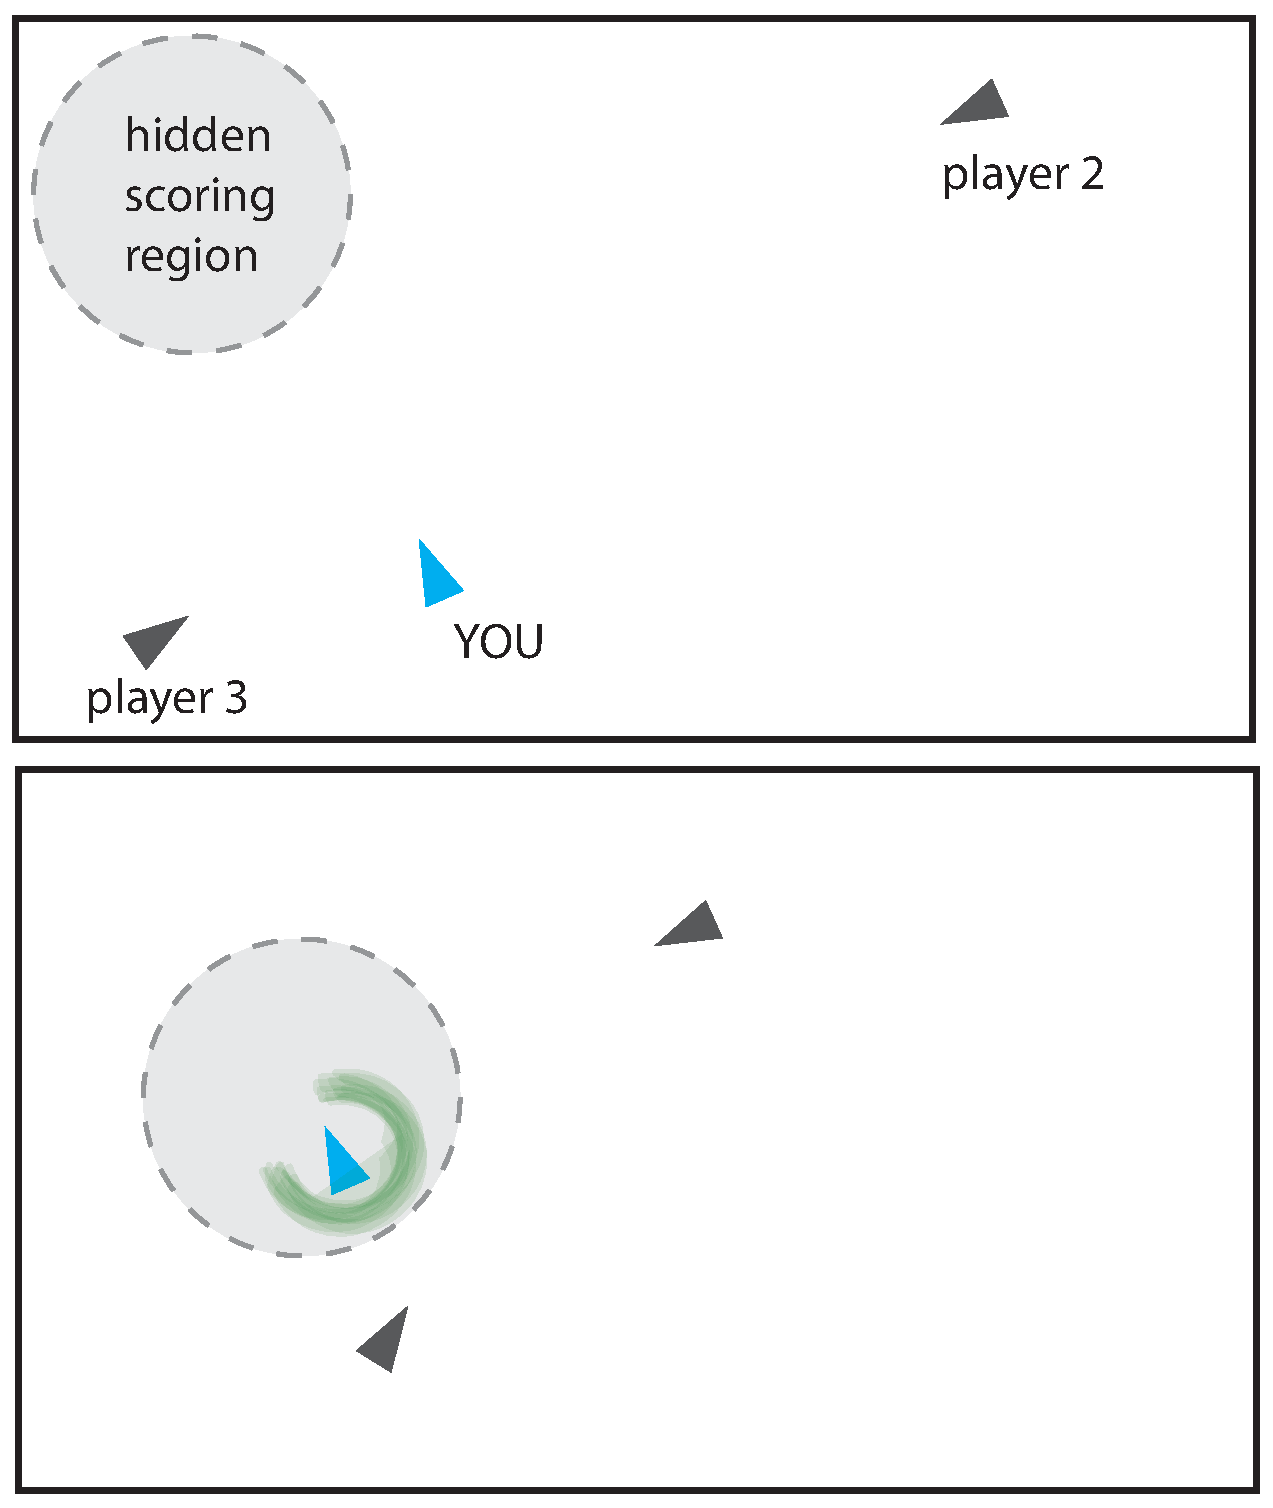
\includegraphics[width=0.6\textwidth]{./figures/experiment1_design.pdf}
  \hspace{0.1cm}
  \caption{Example states of the multi-agent tracking task used in Exp. 1. Hidden scoring region is shown in grey, slowly drifting over time. Bottom frame shows participant receiving a bonus reward upon entering the region. The halo indicating this bonus was only visible to the participant inside the region, and not to the other participants.}
  \label{fig:score}
\end{figure}

Participants controlled avatars in a rectangular virtual environment by clicking and using two keyboard keys. 
Avatars automatically moved forward, and clicking within the playing area instantly oriented the avatar to move toward the clicked location. 
Participants could hold the ``a" key to accelerate or hold down the ``s" key to stop.  
We designed the environment as a multi-agent tracking task (Fig. \ref{fig:score}).
The score that agents obtained at each location at each point in time was determined by an underlying ``score field,'' which was generated by slowly moving a circular ``spotlight'' along paths between randomly chosen locations.
This field was hidden from participants, who only had access to the score at their current location. 
We pre-generated 5 such score fields, so multiple groups were randomly assigned to the same underlying field.  

These simple score fields were binary (i.e. 1 inside the circular scoring region and 0 everywhere else), so we showed participants binary feedback about their current score.
When an avatar entered the circular region, it was surrounded by a salient sparkling halo and the border of the playing area turned green (see supplementary Fig. S1 for screenshots). 
Critically, this feedback was only visible to the participant controlling that avatar; participants did \emph{not} directly observe whether other participants were in the scoring region. 
They could only see the spatial location and orientation of other participants, updating in real time.

After successfully completing a comprehension test, participants were redirected to a waiting room.
Each waiting room was assigned a group size between 1 and 6, and the game began as soon as the target number of participants was reached, or after 5 minutes of waiting, whichever came first.
Participants then played a single continuous game lasting for 5 minutes, and were paid a bonus proportional to the total score they (individually) accrued.

See Appendix B in Supplementary Materials for further details of our stimuli and procedures.

\begin{figure}[t!]
  \centering
  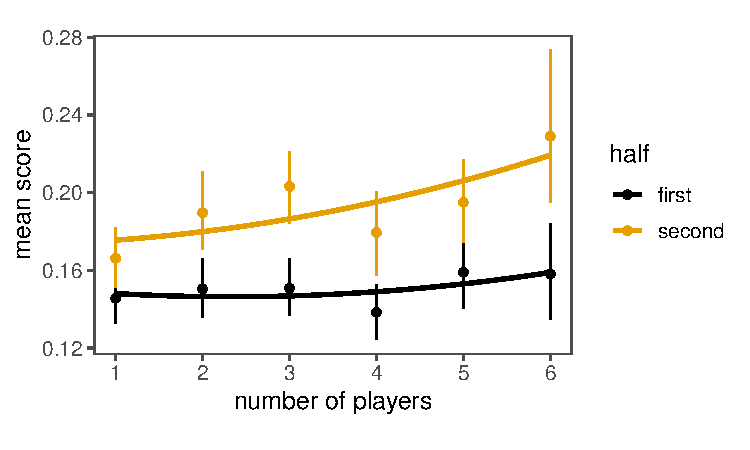
\includegraphics[width=0.8\textwidth]{./figures/performance-summary-exp1.pdf}
  \caption{Mean performance of human participants in each half of Experiment 1 as a function of group size. Larger groups saw significant gains in performance. Error bars are 95\% bootstrap confidence intervals using the group as the primary bootstrap unit. %\andrew{Ok, so going back to my other comment (sensing vs learning), this suggests the collective sensing is learned. Is that new/cool/unique, or am I just tired?}
  }
  \label{fig:exp1_performance}
\end{figure}

\subsection{Results}

We hypothesized that individuals in larger groups would be able to achieve higher scores on average than individuals in smaller groups. 
We also hypothesized that the advantages of larger groups would accrue later in the game, when participants had adjusted to the mechanics of the environment and the behavior of the other participants.
To test these hypothesis, we examined performance during each half of the 5-minute session. 
In cases where one or more participants were disconnected or removed, we measured the size of the group at the end of the session.
We constructed a mixed-effects regression predicting each individual participant's average score over the time period, including fixed effects of period (first vs. second half), the continuous number of participants in their environment (one through six), and their interaction.
We also included random intercepts for each group and each of the five underlying score fields.
First, we found a main effect of practice: scores were significantly higher on the second half of the session ($b = 2.1,t=-10.8, p < 0.001$).
However, we also found a significant interaction with group size: while performance on the first half was similar across group sizes, the performance of each individual on the second half significantly increased in larger group sizes from a score of 0.16 in groups of 1 to 0.24 in groups of 6 ($b = 0.33$, $t = 2.8$, $p = 0.004$; see Fig. \ref{fig:exp1_performance}). 

\section{Experiment 2: Evaluating copying strategies}

What cognitive abilities allowed humans in Experiment 1 to benefit from collective intelligence even when the payoff information of other agents is not directly accessible?
We hypothesized that human behavior in this environment is driven by two underlying strategies: (1) independent exploration and (2) precise, targeted copying based on social inferences about success. 
These hypothesized strategies rely on cognitive abilities allowing humans to infer ``who knows'' about high-scoring locations based on outward behavioral traces (e.g. slowing down or stopping in a region) and also to inhibit social influence to act independently when appropriate.

The design of Experiment 1 made it challenging to disentangle these strategies.
For example, we were interested in analyzing participant clicks to detect signatures of selective copying, but because there was a unique `spotlight' at each point in time, different copying strategies were confounded: participants who were already obtaining reward and trying to stay inside the spotlight were, by necessity, clicking close to other participants who were obtaining reward, even if they were not intentionally copying them.

For our second set of experiments, then, we designed a sequence of controlled scenarios that are more diagnostic for testing the use of these different strategies.
We placed participants into an environment with artificial agents that we designed, rather than other humans, and we manipulated the location of the score field to estimate the probability of copying different agents under different conditions.

For conceptual clarity about our design and analysis, it is helpful to define three broad `states': exploring, exploiting, and copying \cite<e.g.>{rendell_why_2010}.
We define \emph{exploiting} as selecting an action that maximizes the expected score given the agent's current knowledge of the environment, i.e. staying close to a known location of the spotlight. 
We define \emph{copying} as forward motion, sometimes accelerated, toward the location of another agent. 
We define \emph{exploring} as selecting an action that has an unknown outcome, often moving to a region without other agents. 
In this environment, exploiting, exploring, and copying behavior were associated with distinct and recognizable movements.
Our hypothesized strategies can be operationalized as selective deployment of these three states: exploiting rather than copying or exploring when one is in a high-scoring region, and copying rather than exploring in low-scoring regions only when it can be inferred that another agent is receiving a high score, based on outward behavioral signatures.

\subsection{Methods}
\subsubsection{Participants}

We recruited 28 unique participants from Amazon Mechanical Turk.
All participants were from the United States.

\subsubsection{Stimuli \& procedure.}

As in our first experiment, participants were given control of an avatar to explore a virtual environment and were rewarded based on their location according to a hidden ``score field.'' 
The interface and controls were the same as in Experiment 1, but the procedure differed in several ways. 
Instead of a single 5-minute session, we designed a sequence of shorter scenarios that were informative for distinguishing between several different potential mechanisms that could be used in the game. 
These scenarios carefully controlled score field dynamics and bot behaviors. 

\begin{figure}[t!]
  \centering
  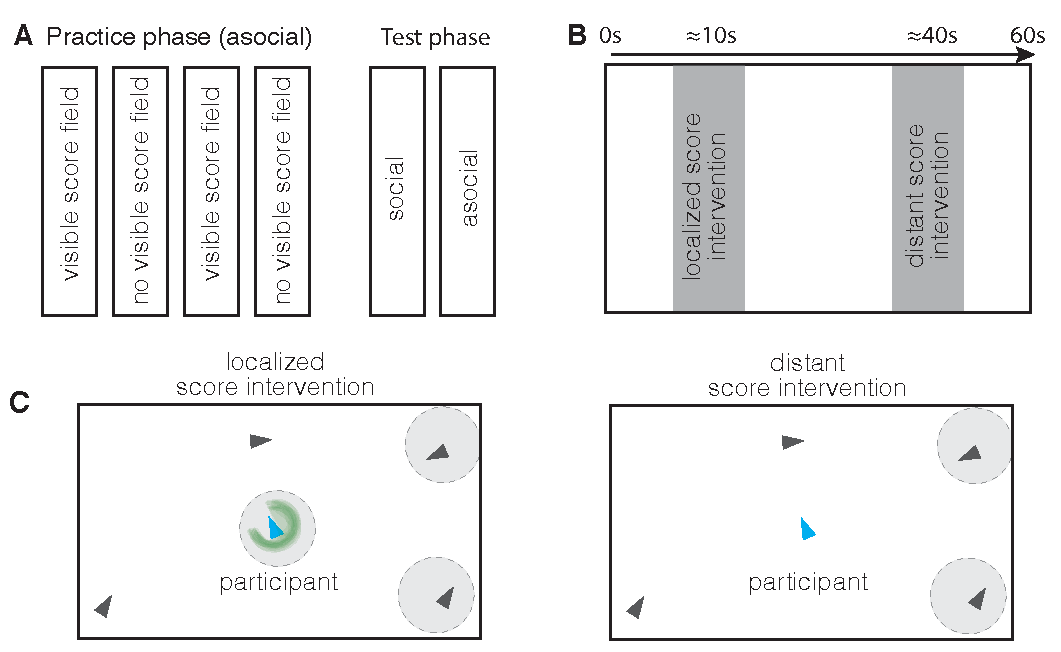
\includegraphics[width=1\textwidth]{./figures/exp2_design.pdf}
  \caption{Design of Experiment 2. (A) The timeline of the test round involves a baseline condition with no score field, and two causal interventions on the score field beginning at approximately 10 seconds and 40 seconds. (B) These interventions manipulate the location of the score field to ensure the participant is receiving high reward or not, respectively, while a subset of other agents are receiving high reward.}
  \label{fig:exp2_design}
\end{figure}

After four one-minute practice rounds, where no other agents were present (see Appendix C in our Supplementary Materials for more details), participants were placed in two one-minute test rounds that were the focus of our analyses. 
In one of the two test rounds, no other agents were present (non-social condition), and in the other there were four bots in the environment (social condition). 
We randomized the order of social and non-social conditions across participants. 
Each of these rounds was further divided into three conditions, where we causally intervened on the score fields to better test our hypotheses about exploring, copying, and exploiting behavior. 

For the \emph{baseline} condition, there was no score field. During these times, all the bots were randomly exploring, with two randomly exploring along walls (in association with the wall score field dynamic) and two exploring the center region (associated with the random walk score field dynamic). 
Around the ten second mark and the forty second mark in each round, we introduced the two high scoring regions into the game (see Fig.~\ref{fig:exp2_design}A).
In the \textit{distant intervention} condition, we superimposed the wall-following and random-walk score field patterns to create a bi-modal dynamic score field. 
We centered one high scoring region on a wall-following bot and one high scoring region on a bot in the center region. 
In the \textit{local intervention} condition, however, we also placed a high scoring region on the \emph{participant}, wherever they were. 
In this condition, they automatically received a high score for roughly the ten second duration that the high scoring regions were present (see Fig.~\ref{fig:exp2_design}B). 
We randomized the order in which these two interventions appeared.

Bots followed a simple selective copying algorithm. 
They were programmed to immediately stop upon entering a high-scoring area.
If other bots in the environment were stopped, they copied them, and explored non-socially when no other bots were stopped.
The wall-following bots only copied other wall-following bots, and the bots in the center region similarly only copied each other.
Bots were not responsive to the participant's behavior, only to each other.
In the non-social round, we simulated the same bots, so that the distribution of score field positions was the same across the two conditions. 
The score field manipulation was triggered for the bots approximately two seconds after it was triggered for the participant in the local intervention condition. 
We offset the onset in order to ensure that participants were already aware of their own score before observing any reward-related bot behavior.

% \subsection{Hypotheses}

% \paragraph{Testing social behavior:} We included the non-social trial condition as a control to help us adjust our statistical analysis of behavioral mechanisms to account for behavior that looks social by chance. 

% \paragraph{Testing exploring behavior:}  With the blank score field manipulation we are able to test if participants explored randomly or copied other participants when nobody in the game was receiving a high score. 

% \paragraph{Testing copying behavior:}  The targeted score field manipulations allowed us to test whether the participant would preferentially click towards the exploiting bots, and if they had any preference for the bots who were operating on the same score field dynamics the participant had practiced on.

% \paragraph{Testing exploiting behavior:}  The purpose of the localized score field manipulation was to see whether participants would exploit when they receive a high score, regardless of what else was going on in the environment.

% \begin{table}[]
% \begin{tabular}{r|c|c}
%                       & Participant receiving reward & Participant not receiving reward  \\ \hline
% Selectively copy  & Eagerness                   & \multicolumn{1}{c|}{Selectivity} \\ \hline
% Indiscriminately copy &  \multicolumn{2}{c|}{Independence}  \\ \cline{1-3} 
% \end{tabular}
% \caption{Table of terminology for behavioural patterns?}
% \label{tab:qual_scoring_defs}
% \end{table}

\subsection{Results}

To analyze our data from this experiment we use a mixed methods analysis involving both a qualitative coding approach and a quantitative analysis of behavioral traces and click data. 

\subsubsection{Qualitative Coding Results}

For our qualitative analysis, two authors manually coded videos of our 28 participants. We coded for three behavioral signatures --- \emph{selectivity} in copying exploiting bots, \emph{eagerness} in copying other agents, and \emph{independence} in exploration --- on a scale from 0 to 1. \emph{Selectivity} was defined by examining behavior during the distant condition, when the participant was not themselves receiving a reward but another agent was: selectivity was coded as a preference for moving towards agents who were exploiting, as opposed to moving toward agents who were exploring or copying. This behavioral signature marks participants as selectively copying agents who are exploiting the high scoring regions.
\emph{Eagerness} was defined by the same preference for moving toward exploiting agents during the local condition when the participants were themselves receiving a high score, such that their copying behavior was not contingent on their own state. Eager agents copy even when they could be exploiting the high scoring region they have already identified.
Finally, \emph{independence} was defined by reverse-coding a preference for moving towards agents who were \emph{not} stopped, at any point in the task---i.e., indiscriminately copying other agents. This signature primarily captures whether participants were preferentially moving toward other agents during the periods when there was no score field active, thus we interpret low prevalence of this signature as high independence. 
The endpoints of the scale roughly represented the proportion of time the participant spent displaying the behavior in question compared to the potentially available opportunities to do so. 

The two coders achieved a correlation of $r = 0.75$ for selectivity, $r = 0.55$ for eagerness, and $r = 0.60$ for independence. The coders resolved disagreements in our codes by averaging. 
First, we found that a substantial fraction of participants display selective copying behavior and independence (Supplemental Fig. S2). 
%\todo[inline]{rdh: Is it appropriate to use 0.5 as the null threshold? Do we think that midpoint is meaningful, since even lower numbers, e.g. 0.2, were indicative of some level of these signatures? Maybe should be comparing to a null of 0?}
We found that 71\% of participants had an average selectivity rating of at least 0.5, and 86\% had an average independence rating above that level. 
These proportions were significantly greater than 50\% using a two-sided binomial test, $p = 0.036$ and $p = 0.001$, respectively.  
In comparison, only 1 participant (4\%) was coded as eager at that level, which was significantly less than 50\%, $p < 0.001$.
These qualitative results show that participants appeared to selectively copy stopped agents when they themselves were not receiving reward, but otherwise mostly inhibited social influence.


\subsubsection{Quantitative Behavioral Results}

\begin{figure}[th!]
    \centering
    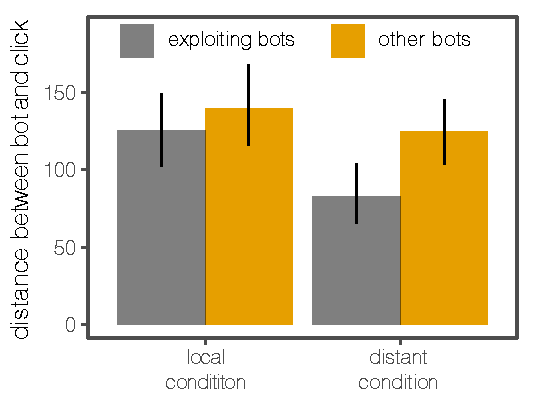
\includegraphics[width=0.8\linewidth]{figures/proximity.pdf}
    \vspace{-1em}
    \caption{Participants selectively copy other agents who appear to be exploiting, but only when they themselves are not receiving reward (i.e. the distant intervention condition). We operationalized copying in terms of the spatial distance from the click to the bot's location, so lower distance is evidence of copying. Error bars are bootstrapped 95\% CIs.} %\todo[inline]{check is nonsocial makes it look better. otherwise relegate to appendix}}
    \label{fig:proximity}
\end{figure}

Next, we tested these same hypotheses quantitatively using data we recorded of participants' locations and the state of the environment at each time step of the experiment.
We operationalized copying using participant clicks.
Because clicking near another agent moved them closer to their target's location, and success is based on spatial location, we examined the proximity of each click to other agents.
To test whether participants selectively copy agents who appear to be exploiting, we computed both the distance to the nearest agent who is stopped, and the nearest agent who is not stopped.
We then compared copying rates across the two score field conditions: we predicted that participants would inhibit selective copying in the \emph{local} condition, when they automatically received a score in their current location, relative to the \emph{distant} condition, where the score field was only placed on top of artificial agents.
To test this prediction, we constructed a mixed-effects regression model predicting the proximity of each click to the nearest agent as a function of experimental condition (local vs. distant), visible behavior (exploiting vs. not exploiting), and their interaction.
We included the maximal random effects supported by our within-participant design, allowing random intercepts, main effects, and interactions at the participant-level.
We found a significant interaction, $b = 47.6, t = 2.5, p = 0.02$, indicating a selective preference for copying other exploiting agents, but only in the condition when the participant was not themselves receiving a reward (see Fig. \ref{fig:proximity}). 
To control for the possibility that this result is a product of generic biases in the spatial pattern of clicks, rather than the use of social information, we conducted the same analysis on clicks in the \emph{non-social} condition, where no artificial agents were visible but the underlying score field dynamics were the same. 
In other words, this condition allows us to examine the proximity of clicks to where other agents would have been. 
We found no significant interaction in this condition, $b=30.1,~t=1.4,~p=0.18$.
A stronger test of this comparison would be the three-way interaction in a single model testing whether the interaction estimated in the social condition differed significantly from the one in the non-social condition.
This three-way interaction was not significant, $b=20.1,~t=1.2,~p=0.19$. 
Exploring the baseline variability of clicks in non-social environments is likely to be a fruitful target for future work using a more highly-powered sample. 

\section{Experiment 3: Generalizing to more complex environments}

To generalize our understanding of these findings to more complex environments, and to more explicitly compare our findings to the nonhuman animal literature, we conducted a final experiment using the materials designed by \citeA{berdahl_emergent_2013} to examine collective sensing in fish.
These environments are significantly more complex than the binary spotlight and border environments we used in Experiments 1 and 2.
They require agents to use continuous gradients to navigate noisy and fluctuating score fields.
We manipulated the level of noise across different groups, predicting that the cognitive abilities discussed in the previous sections may be less reliable under noisier conditions. To test that the social learning strategies identified in the previous experiments also generalize to different external behavioral signatures, we also modified several other aspects of the experiment interface, including the movement controls.
This small change created a different behavioral cue of success (spinning in place rather than stopping or slowing), which agents equipped with social inference mechanisms should be able to use for selective copying just as effectively as participants in the previous experiments.

\subsection{Methods}
\subsubsection{Participants}

We recruited 563 unique participants from Amazon Mechanical Turk to participate in our experiment.
All participants were from the United States.
After excluding 72 participants due to inactivity or latency, and 6 others for disconnecting in the first half of the game, we were left with usable data from 437 participants in 224 groups.
113 individuals (63 groups) were in the low noise condition and 324 individuals (161 groups) were in the high noise condition. 
These groups ranged in size from one to six individuals.  
Since only one group of size six completed the task without disconnections, we ignored this group in our analysis.

\subsubsection{Stimuli and Procedure}

%Based on the method reported by Berdahl et al., we added 

Our primary change from Experiments 1 and 2 was switching from a binary score field to a more complex, gradient score landscape.
These more complex fields were generated using the method reported by \citeA{berdahl_emergent_2013}. 
We began with the same randomly moving ``spotlight'' of high value as before. 
However, we then combined the spotlight with a field of spatially correlated, temporally varying noise.  
By manipulating the proportional weighting of the noise field and the spotlight, we generated two different conditions, corresponding to two of the noise levels used by \citeauthor{berdahl_emergent_2013}. 
In the \emph{low noise} condition, the spotlight was weighted strongly compared to the noise field (10\% noise), with the noise field providing minor background variation (see Supplemental Fig. S3, left). 
In the \emph{high noise} condition, the weighting of the noise field was increased (25\% noise), providing more extreme fluctuation outside of the spotlight (see Supplemental Fig. S3, right).
To decrease variability and increase statistical power, we generated only four distinct score fields per noise level, so multiple groups experienced the same fields.  

In addition to these more complex score fields, we made several adjustments to the interface.
First, rather than showing their current score as binary---a glowing halo around the participant when inside the spotlight---their score was presented as a percentage at the top of the playing area (see Supplemental Fig. S5 for a screenshot).
Second, rather than clicking to change direction, participants controlled their avatars using their keyboard. 
The left and right arrow keys were used to turn (at a rate of $40^\circ$ per second) and the
spacebar was used to accelerate. 
Unlike before, we did not provide a mechanism to stop completely.  
Given the closer relation to \citeA{berdahl_emergent_2013} in this experiment, it is also relevant that the speeds of the avatars and the playing area dimensions ($480 \times 285$) throughout all of our experiments were matched to those reported by Berdahl et al.; in this experiment, we additionally used the same total task length of six minutes.
The procedure was otherwise identical to Experiment 1.

\begin{figure}[t!]
  \centering
  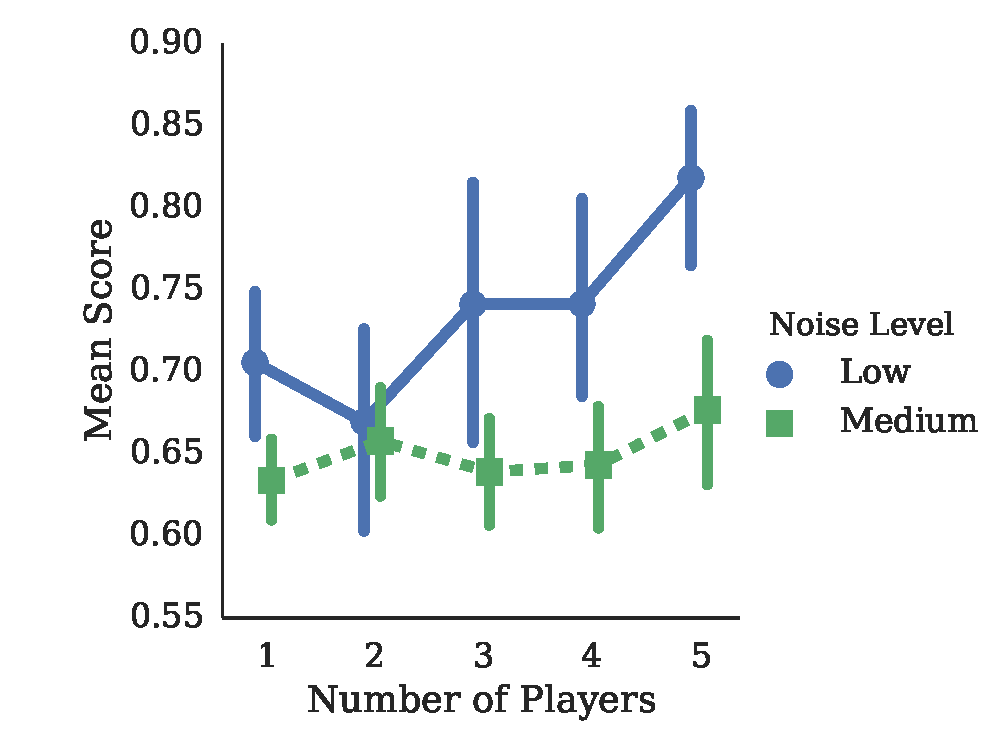
\includegraphics[width=0.95\textwidth]{./figures/performance-summary}
  \caption{Mean performance as a function of group size under different noise conditions.  Error bars are 95\% bootstrap confidence intervals using the group as the primary bootstrap unit.}
  \label{fig:performance}
\end{figure}

\subsection{Results}

Our analyses focus on two primary questions: (1) how does the introduction of a noisier environment affect collective performance, and (2) how do the selective social learning strategies identified in Experiment 2 play out in such an environment, when inferences about the success of other agents may be less reliable?

\subsubsection{Effects of noise on collective performance}

We begin by analyzing patterns of collective performance across groups of different sizes and across the different noise conditions.
As our measure of performance, we computed the average score obtained by participants over each half of the experiment.
To test effects of performance, we constructed a linear regression model with main effects of group size (1 through 5), half (`first' vs. `last')  and noise condition (`low' or `high'), as well as their interactions.
All three main effects were significant: all else being equal, scores tended to increase with group size, $b=1.4,~t=3.9,~p <0.001$, were higher in the second half compared to the first half, $b=2.7,~t=5.2,~p<0.001$, and were higher in the low-noise condition than the high-noise condition, $b=4.1,~t=-7.8,~p<0.001$.
The only significant interaction was between noise condition and group size, $b=0.89,~t=2.4,~p=0.018$, indicating a stronger effect of group size in the low-noise condition than the high-noise condition (see Fig.~\ref{fig:performance}).
We also conducted a mixed-effects regression including random intercepts for each group (i.e. controlling for possible correlations between participants in the same group) and for each score field (i.e. controlling for the possibility that some randomly generated score fields were more difficult than others). We found that the main effects of group size, game half, and noise condition were robust $(p=0.037,p=0.001,p<0.001$, respectively) but the interaction was no longer significant, $p=0.23$, with the group-level random intercept accounting for the bulk of the additional variance. We suspect this discrepancy is due to dramatic loss in power to detect an interaction after shifting from the participant-level unit of analysis to the group-level unit of analysis, especially given imbalances in sample sizes across noise conditions. Thus, we believe this effect merits further investigation.
% We found a significant interaction between group size and noise condition ($b = $). 
% As in Experiment 1, performance in the low noise condition increased significantly in larger groups.  
% However, there was less improvement with larger group size in the high noise condition (see \ref{fig:performance}). 
% Moreover, examining the random effects also revealed larger variability due to score field in the ``high'' noise condition than the ``low'' noise condition.
% One particular score field in the high condition displayed a significant effect of group size, while none of the others do. 
% Qualitative inspection revealed that this particular score field seemed to share spatial properties more similar to the low noise score fields (e.g. fewer local maxima).  
% \todo[inline]{Double-check this?}
Overall these results indicate an important role of the environment in group success: under low noise, larger groups perform systemically better than smaller groups, similar to the effect found in Experiment 1, yet this advantage appears to be weaker under high noise.
%The improvement we found in the low-noise condition contrasts with the lack of any improvement found by \citeA{berdahl_emergent_2013} in fish groups at the same sizes.
%The effect of noise also contrasts with the apparent invariance to noise conditions found in fish behavior.

\subsubsection{Analysis of social learning strategies}

In order to understand the mechanisms that may have contributed to effects of noise on collective performance, we more closely analyzed the underlying behavior of the participants in our games.
While we relied on click data as a useful measure of copying in Experiment 2, here used a simple \emph{state-based} representation of participant behavior based on their keyboard actions.
We empirically determined the state of each participant at each point in time --- exploring, exploiting, or copying --- using a simple set of hand-specified criteria (see Appendix D in our Supplementary Materials for details).
All of these criteria depended only on information that was observable to participants in the game (i.e., the filters do not depend directly on the hidden scores of other individuals), and hence we can use these states as proxies for what participants might be able to infer.
Additionally, because the states are not defined in terms of score values, we can meaningfully quantify the relationship between state and performance.

\begin{figure}[t!]
  \centering
  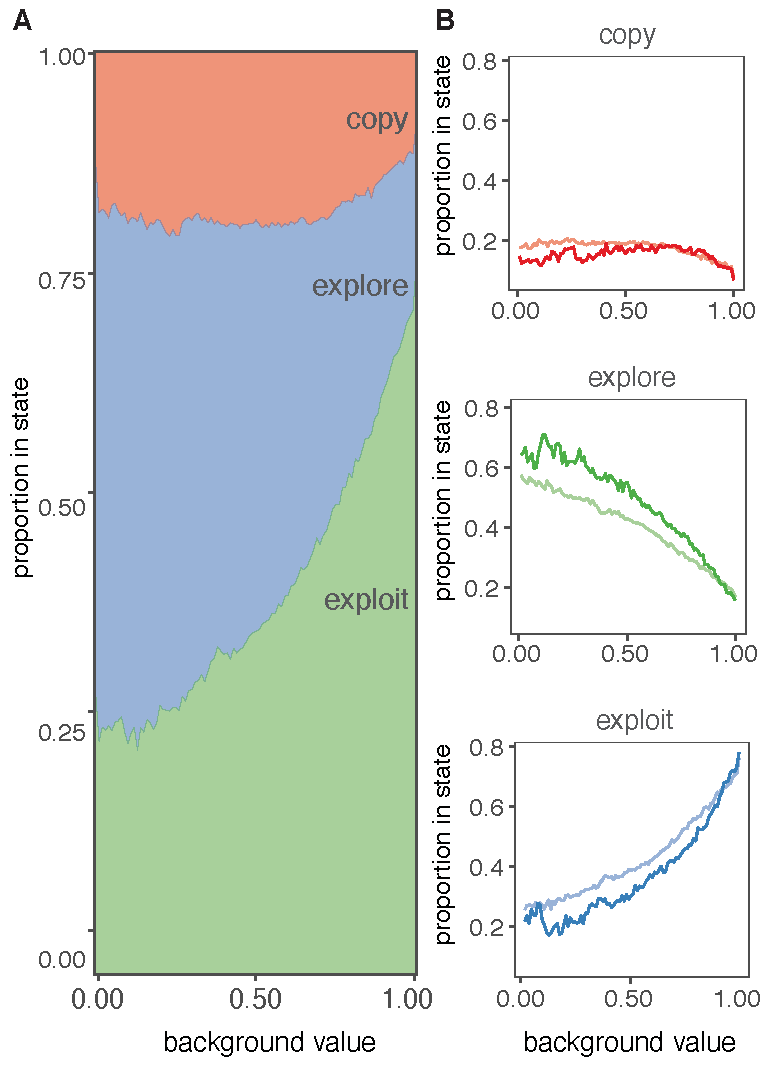
\includegraphics[width=0.6\textwidth]{./figures/new_states}
  \caption{(A) The probability of an individual being in a particular behavioral state as a function of the individual's score, combined across both conditions. (B) Participants tended to begin exploiting at lower background values in the high-noise condition, leading to less copying and exploration.}
  \label{fig:states}
\end{figure}

We now proceed to use these state classifications to analyze the behavioral strategies used by participants in our game.
First, in line with our finding in Experiment 2 that participants inhibit copying when they find themselves in high-scoring regions, we predicted that the probability of the exploiting state would increase as participants receive higher scores.  
To test this prediction, we constructed a logistic mixed-effects regression model predicting the probability that each individual is in the `exploiting' state at each time step. 
We included fixed effects of their current background score and noise condition, as well as their interaction.
We also included random intercepts for each group and score field.
First, we found a strong main effect of the current score: regardless of noise condition, participants are significantly more likely to exploit in higher scoring locations than in lower scoring locations, $b=3.2,~z=310,p<0.001$  (see Fig.~\ref{fig:states}A).
Selective exploiting is clearly adaptive, as participants will tend to remain in high scoring regions but quickly move away from low scoring regions either by exploring independently or by copying other individuals.
At the same time, strategies differed dramatically across noise conditions: we find a significant main effect of noise, $b=0.3,~z=3.7,~p<0.001$, indicating that participants are significantly more likely to engage in exploitation in the high noise condition at all background values.
We also found a significant interaction between condition and background value, $b=-0.3,~z=-33,~p<0.001$, indicating that the increased likelihood of exploitation is especially pronounced at lower background values (see Fig.~\ref{fig:states}B).
Similar regressions predicting the probability of `copying' and `exploring' states found that participants were also \emph{less} likely to be exploring, $b=0.26,~z=27,~p<0.001$, and \emph{more} likely to be copying, $b=0.08,~z=6.2,~p<0.001$, at lower point values.

A lower threshold for exploitation may also help explain gaps in collective performance across noise conditions. 
First, a willingness to exploit at lower point values may, by definition, lead to lower overall performance. 
Second, it may make copying less effective, preventing social learning mechanisms from improving performance in larger groups.
That is, if participants are willing to exploit at lower background values, then external cues of exploiting (i.e. ``spinning'' behavior) will provide statistically weaker evidence of underlying success.
To test this hypothesis, we identified all of the events in our dataset where one participant copied another and measured the current score of the target of copying.
We found that targets of copying tend to be in lower scoring regions in the high-noise condition, $d=0.08,~t=4.02,~p<0.001$.
These results clarify the interaction between human social learning strategies and environmental conditions, and raise interesting questions about the robustness of social inference based copying.
We discuss these questions in more detail below.
%In Experiment 2, we found that participants did not copy indiscriminately but were able to selectively copy participants receiving high rewards, even though these rewards were not directly visible. 
%In this experiment, we likewise examined the scores of the participants who are being copied.
% Moreover, as shown in Figure \ref{fig:proportion}, groups that contain individuals who focus their copying behavior on higher scoring individuals achieve significantly higher performance in our task (slope: 0.2639, 95\% CI: $[0.145,  0.383]$). 
% A participant who is able to accurately infer whether another participant is receiving a high score may be able to achieve higher performance on our task by leveraging these inferences to more effectively copy others.

\section{Discussion}

%summary
Our experiments established that human groups display collective intelligence -- in the form of emergent sensing -- during a dynamic spatial search task.
%In agreement with past experiments on non-human animals \cite{berdahl2018collective}, larger groups were better able to sense and respond to their environment.
Individuals in larger groups were better able to sense and respond to their environment.
Further, we were able to uncover the mechanisms driving the emergent sensing:
individuals, who only had access to extremely local (scalar) information about the spatial resource field,  were able to use information inferred from the behaviors of other individuals to develop a non-local measure of the hidden underlying resource field. We confirmed that selective social learning relying on simple agent-reasoning, rather than indiscriminate copying, was employed to enable this intelligent collective behavior. We also confirmed that these abilities and behaviors were sustained in a more complex experimental environment.
%Further, we were able to uncover the mechanisms driving the emergent sensing.
%Even though individuals only had access to extremely local (scalar) information about the spatial resource field, they were able to use information inferred from the behaviors of other individuals to develop a non-local (gradient) measure of the hidden underlying resource field.
The inference drawn appeared to be rapidly learned during the experimental trials and may be unique to humans, suggesting that human's meta-cognitive reasoning and agent reasoning abilities, such as theory of mind, may allow collective intelligence to rapidly emerge in novel settings.

%The inference involved may be unique to, or at least more common in, humans and appears to require on-the-fly (in situ?) learning.

\paragraph{Comparison to Prior Work.}

%comparison to fish I
Our study design was inspired by a collective sensing task used in the animal behavior literature, particularly the one proposed for groups of fish by \citeA{berdahl_emergent_2013}. 
We found similar improvements in performance as a function of group size in humans, suggesting that the general phenomenon of collective sensing persists across different species \cite{berdahl2018collective}.
However,  the mechanisms driving the collective sensing appear to be very different between the fish and humans. 
In fish schools, resource-level-dependant speed modulation induced group-level turning toward high-resource areas, while humans were led to these high-resource areas via strategic copying based on the inferred performance of others.
These differences support recent work in social learning \cite{wisdom_social_2013, mcelreath_beyond_2008}, which find flexibility in the strategic deployment of imitation in humans. Appendix A in our Supplementary Materials provides one plausible model that could describe the form of selective copying we observe.

%comparison to fish II
Differences in the group performance versus group size between fish and humans reveals a potential trade-off between the underlying mechanisms. 
First, we found that humans were able to achieve increases in performance at much smaller group sizes than fish. 
Humans had substantial improvements in performance at just five participants, while schools of fish only showed really significant improvements at groups of 64 and 128.  
Second, while there was no difference in the effect of group size across different environmental noise levels for fish, we found that in the small-group regime we considered, the benefits of larger group sizes only accrued in low-noise conditions for humans.
Taken together, these two differences show that the emergent sensing in humans may be more powerful than that found in fish, but the mechanism used by the fish is more robust to noisy environments.
However, we note that it is difficult to make quantitative comparisons between human performance to the performance of fish given the differences between the perceptual and motor abilities of fish in a tank and those available to participants in our simulated environment. Yet our study nonetheless raises interesting questions about the potential trade-offs between differences between mechanisms for collective intelligence.











%Our study design was inspired by collective sensing tasks used in the animal behavior literature, particularly the one proposed for groups of fish by \citeA{berdahl_emergent_2013}. 
%Our use of the same resource fields as this fish study allows us to make direct qualitative comparisons between humans and fish; however, we note that it remains difficult to make broad quantitative comparisons of human performance to the performance of fish given the differences between the perceptual and motor abilities of fish in an tank and those available to participants in our simulated environment.
%We found similar improvements in performance as a function of group size in humans, suggesting that the general phenomenon of collective sensing persists across different species \cite{berdahl2018collective}.
%Although driven by a very different mechanism, the improvements in performance as a function of group size in humans was consistent with that in fish, suggesting that the general phenomenon of collective sensing persists across different species and mechanisms \cite{berdahl2018collective}.
%However, \andrew{perhaps unsurprisingly,?} the mechanisms driving the collective sensing appear to be very different between the fish and humans. 
%In fish schools, resource-level-dependant speed modulation induced group-level turning up gradients, while in humans, strategic imitation based on the inferred performance of others led individuals to resource-rich areas \cite{wisdom_social_2013, mcelreath_beyond_2008}.


%%Fish exhibited mild improvements in average performance at groups of 16 and more substantial improvements at groups of 64 and 128. In contrast, we observed significant improvements in human performance at just five participants. This difference in group size needed to achieve effective collective sensing suggests that the flexible copying mechanism employed by humans 


%First, we found that humans were able to achieve increases in performance at much smaller group sizes than fish. 

%Second, while there was no difference in the effect of group size across different environmental noise levels for fish, we found that in the small-group regime we considered, the benefits of larger group sizes only accrued in low-noise conditions for humans.







\paragraph{Social Learning in Non-human Animal Groups.}


%comparison to animals more generally
Our work demonstrates consequences of fast social inferences in human groups. In contrast, the status of similar abilities in non-human animals remains more controversial.
The use of fast social inferences in human groups may be widespread, but the status of similar abilities in non-human animals remains more controversial.
Across a broad diversity of taxa, both gregarious and non-group-living species use social information when locating resources \cite{danchin2004public} and many examples are consistent with inferential behaviour.
Just as our human participants moved toward others `spinning’ within a reward patch, vultures are attracted to the circling flight of other carrion eaters \cite{kane2014vultures}. 
Bats use odors from the breath and fur of conspecific when deciding where to forage \cite{omara2014frugivorous}
and seem to prefer novel conspecifics, perhaps to inject new information \cite{ramakers2016frugivorous}.
Cliff-dwelling swallows, appear to engage in signalling behavior at food sites \cite{brown1988social,brown1991food}, which effectively externalizes success and draws conspecifics to enhance the efficiency of foraging \cite{torney2011signalling}.
Uninformed fish and rats leave protection to follow trained conspecifics to feeding sites, presumably by responding to the behaviors trained individuals display when anticipating food \cite{reebs2000can,bennett1997socially}.
Despite the prevalence of social information use in foraging animals, and the superficial consistency with inference, it remains unclear whether these cases reflect social reasoning abilities beyond standard operant and respondent conditioning that associates social information with foraging success \cite{galef2001social}.


%more stuff about people literature and theory of mind (Peaks)

%broader impacts (Peaks)







%\newpage
%\section{OLD Discussion (for reference and using bits)}

%\todo[inline]{rxdh: need to revise this summary to state the problem again and say briefly the contribution of each experiment.}
%Our experiments established that people display collective intelligence in a multi-agent tracking paradigm inspired by experiments conducted with fish by previous researchers, and that people display emergent collective intelligence at much smaller group sizes in our environments than fish do in the setup of prior research. \andrew{Should we mention that the underlying mechanism seems to be quite different...}  In our analyses of Experiments 2 and 3, we also confirmed selective social learning strategies allowing people to achieve collective intelligence in this environment.

%\paragraph{Social inference mechanisms in non-human animals.}



%While we focused on the consequences of fast social inferences in human groups, the status of similar mechanisms in non-human animals remains more controversial.
%At least some species, such as cliff-dwelling swallows, appear to engage in signalling behavior at food sites \cite{brown1988social,brown1991food}, which effectively externalizes success and draws conspecifics to enhance the efficiency of foraging \cite{torney2011signalling}.
%Many additional cues of success are available as simple by-products of foraging, such as the sound of eating or (more directly) the scent of food \cite{galef2001social}.
%However, copying based on these cues may be explained by associative learning or other simple biases.

%\paragraph{Comparison to Berdahl et al. (2013).}

%Our study design was inspired by collective sensing tasks used in the animal behavior literature, particularly the one proposed for groups of fish by \citeA{berdahl_emergent_2013}. 
%We found similar improvements in performance as a function of group size in humans, suggesting that the general phenomenon of collective intelligence persists across different species.
%At the same time, we observed some key differences, suggesting that these collective intelligence phenomena may arise from different mechanisms.
%First, we found that humans were able to achieve increases in performance at much smaller group sizes than fish. 
%Fish exhibited mild improvements in average performance at groups of 16 and more substantial improvements at groups of 64 and 128.  
%However, we see significant improvements in human performance at just five participants. 
%Second, while there was no difference in the effect of group size across different environmental noise levels for fish, we found that in the small-group regime we considered, the benefits of larger group sizes only accrued in low-noise conditions for humans.

%This difference in the small-group regime may be at least partially explained by the differences in the mechanism that humans appear to use in this task as compared to fish.

% Golden shiners prefers to spend time in dark areas of the water, presumably to avoid predators.  
% In this task, the researchers studied the effectiveness of the fish at finding the darker areas of the tank as a function of the number of fish participating in the task.  
% The researchers found that average group performance increased significantly as a function of group size, and they identified two simple behavioral mechanisms driving this improvement:
% First, individual fish tended to move more slowly in darker areas. 
% Second, individual fish also tended to turn towards conspecifics.  
% This experiment provides a striking example of a higher level of intelligence at the group level emerging from minimal intelligence at the individual level.

%These differences may partially be explained by the different mechanisms identified in our different studies.
%\citeA{berdahl_emergent_2013} explains collective sensing in fish as an emergent consequence of two more general-purpose processes: (1) the modulation of speed in preferred regions and (2) the general, un-targeted tendency to orient toward other agents.
%These mechanisms have both similarities and differences with the social inference mechanisms we have identified in humans.
%Similar to our finding in Experiment 3 that humans modulate their exploring vs. exploiting behavior based on their current score, fish modulated their speeds based on the level of darkness that they were experiencing.  
%Fish moved slower in their preferred darker areas and faster in lighter areas.  
%And, similar to the copying behavior we observe, fish had a tendency for turning towards other fish.  
%However, the model of fish behavior  did not require any social inference or selectivity. 
%Whereas fish appear to equally weight all nearby conspecifics, humans modulate their copying behavior based on the inferred scores of other participants.
%Additionally, we found that humans strategically deploy \emph{independent} exploration (i.e. explicitly ignoring or moving away from all other agents at times) rather than constantly being pulled toward the locations of other participants. 
%These differences support recent work in social learning \cite{wisdom_social_2013, mcelreath_beyond_2008}, which find flexibility in the strategic deployment of imitation in humans.
%It remains difficult to make broad comparisons of human performance to the performance of fish given the differences between the perceptual and motor abilities of fish in an tank and those available to participants in our simulated environment. 
%Yet our study nonetheless raises interesting potential differences in mechanism.  

\paragraph{Organizational behavior.}

In addition to the recent literature on collective intelligence in nonhuman animal groups, there has been a long line of work studying the factors that predict the performance of human groups in various scenarios \cite{kerr_group_2004,lazer2007network,mason2012collaborative,malone2015handbook,shore2015facts}.  
Our findings are consistent with previous work suggesting that having a larger group is beneficial in complex, uncertain environments \cite{stewart_meta-analytic_2006}.  
Unlike much of this previous work, however, we focus here on the possibility in larger groups of new emergent group abilities and behaviors, and on the mechanisms leading to these emergent properties.

% \paragraph{Meta-cognitive Reasoning.}

% People in our experiments displayed remarkable ability to adapt to the new environment they entered for these experiments. For fish, the ability to
% gain from group performance in these collective sensing tasks is
% likely based on innate behaviors, selected over many generations of
% fish facing exactly this problem over their whole lifespans.  In
% contrast, some of our humans groups, facing this particular problem
% for the first time, appear to have discovered reasonable collective
% sensing strategies in just a matter of minutes. These findings emphasize the importance of meta-cognitive reasoning \cite{heyes2016knows} and flexible agent-reasoning abilities such as theory of mind \cite{woolley2010evidence,engel2014reading} to human collective intelligence.

%Nevertheless, our comparison hints at a superior capacity for distributed cognition in humans, possibly enabled by our ability for theory of mind.

\paragraph{Contextual Factors.}

The picture of collective intelligence in humans and across specifies that is emerging from the scientific literature is that different mechanisms likely give rise to collective intelligence in different species, and that the same can be said even of different types of human collective intelligence displayed in different contexts.  Human collective intelligence on Wikipedia operates in a way that is very different from human collective behavior on social media platforms like Twitter, and both are quite different from the mechanisms of collective intelligence through which bees find new homes or ants scavenge for food. The mechanisms we identify in our experiment are yet another context. Still, the quest continues for what general abilities and principles underlie the range of intricate and sophisticated forms of human collective intelligence \cite{krafft2019simple}, and what distinguish those as a group from the apparently simpler, more swarm-like forms of collective intelligence found in species such as social insects or fish.  Focusing on cognitive abilities rather than behavioral strategies may provide a more domain-general way to understand collective intelligence.

%\paragraph{Conclusions.}
%\todo[inline]{rxdh: this needs to be lightly revised to make sure it flows with rest of argument (currently verbatim from cogsci paper). e.g. the observation about collective memory of actions might be better suited in a previous discussion paragraph?}
%\todo[inline]{pk: scrap if we can't think of something better?}
%Our work sheds light on one of the pressing puzzles of human collective intelligence and human distributed cognition.  What are the abilities that underlie specific mechanisms by which humans establish effective coordinated distributed information processing agents that can accomplish more than any individual alone?  The perspective of group behavior as distributed processing \cite{hutchins_cognition_1995} suggests the importance of communication for collective intelligence because of the importance of communication in distributed systems.  
%Moreover, theory of mind---an enabler of implicit communication---has been shown to be predictive of collective intelligence \cite{woolleyevidence2010,  engelreading2014}.  
%Our work further suggests that one of the roles that theory of mind plays in the emergence of collective intelligence is facilitating implicit communication that allows for coordination on good collective actions. Moreover, our work also suggests that the benefit of a group's coordinating on good actions could be more than simply the benefit to each individual independently.  By combining a natural human tendency for independent exploration with a discerning social awareness, humans appear to be able to fluctuate between exploiting known good actions, independently exploring new options, and intelligently copying the promising choices of other individuals.  A simultaneous combination of these activities by a cohesive group appears to lead to a collective memory of recently good actions from individuals who continue to exploit, and a collective movement towards actions that promise to be good in the near future driven by independently exploring individuals. The reactive distributed sensing ability that appears to emerge from this process may confer a unique benefit to working together in tightly knit groups.
%%who either find new good areas or return to the group.
%% The exploiting
%% core form the body of the group and the exploring individuals form the
%% sticky appendages that drive the group's gradual crawl.

\section{Acknowledgments}

\small

This material is based upon work supported by the National Science
Foundation Graduate Research Fellowship under Grant No. 1122374 to PK
and Grant No. DGE-114747 to RXDH. Any opinion, findings, and
conclusions or recommendations expressed in this material are those of
the authors(s) and do not necessarily reflect the views of the
National Science Foundation.  This material is based upon work
supported by the Center for Minds, Brains and Machines (CBMM), funded
by NSF STC award CCF-1231216.
Special thanks to Colin Torney for providing the code to make the score field gradients, to Hongbo Fang for assisting in validating our qualitative coding, and Robert Goldstone for helpful feedback on the interpretation of our results.

 
\begin{comment}

\end{comment}

\bibliographystyle{apacite}

\setlength{\bibleftmargin}{.125in}
\setlength{\bibindent}{-\bibleftmargin}

\small{
  \bibliography{couzin}
}




\end{document}
